\chapter{Bill of Materials (BOM)\label{sec:BOM}}

A continuación, en la tabla \ref{tab:BOM} se detalla el desglose de todos los componentes necesarios para el desarrollo de este proyecto. Este documento recibe comunmente el nombre de \textit{Bill Of Materials} y permite realizar una estimación aproximada del coste del producto final.

\begin{table} [H]
\centering
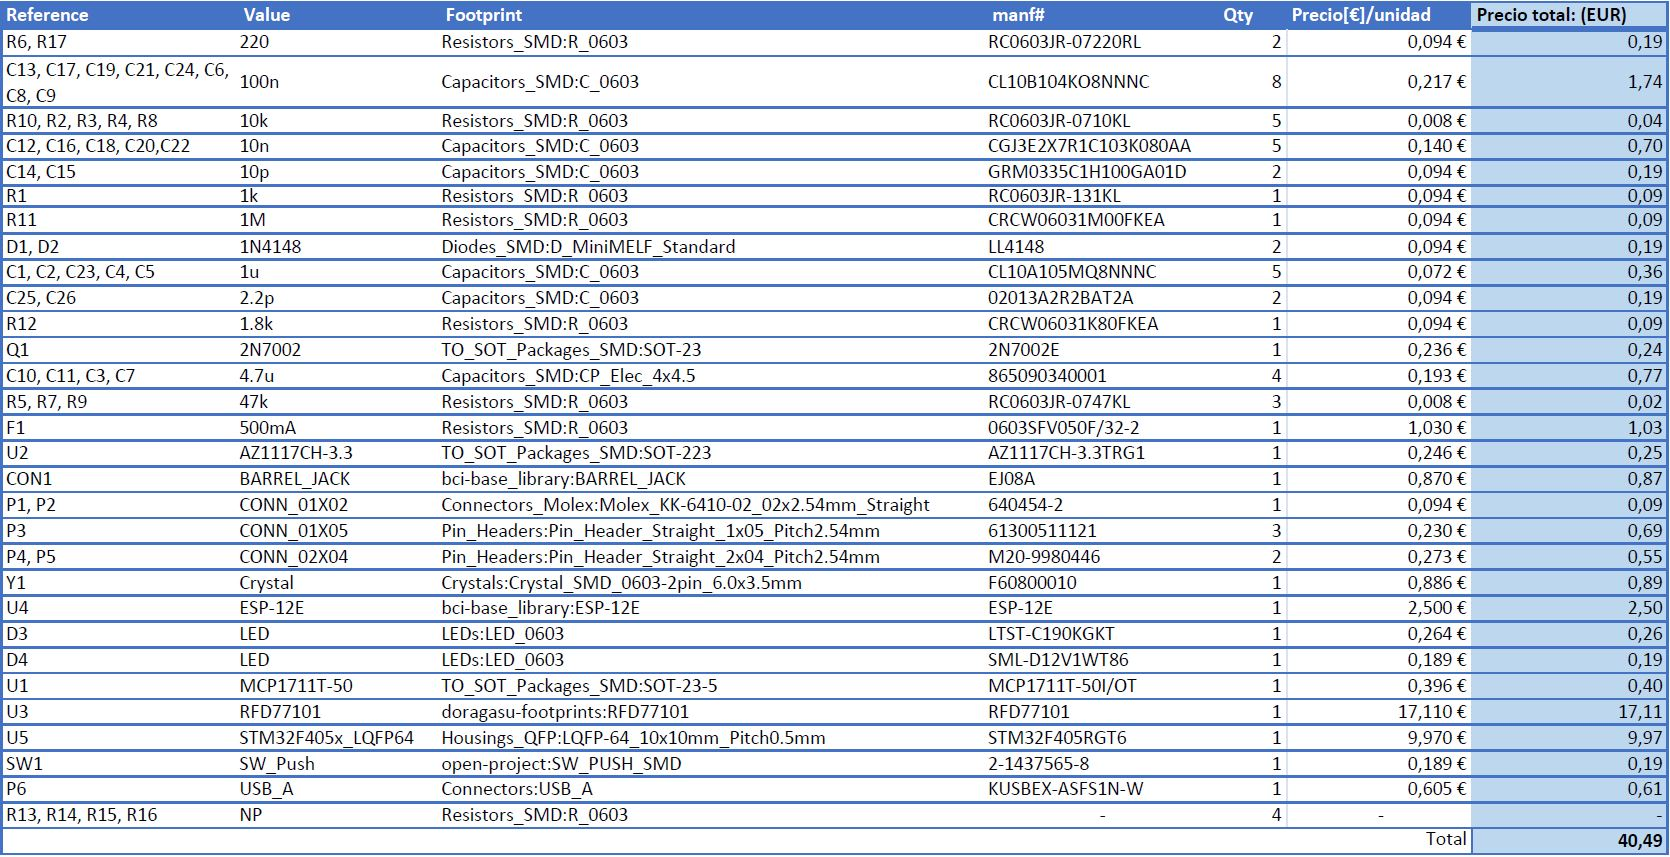
\includegraphics[width = 16cm]{BOM}
\caption{BOM - Bill of Materials}
\label{tab:BOM}
\end{table}

El coste final contando exclusivamente los materiales asciende a 40,49€. 

\clearpage

Es importante destacar que el coste de la tarjeta de procesado no sustituye al de la tarjeta de adquisición sino que lo complementa. Si se desea recrear este proyecto desde cero será imprescindible comprar todos los componentes y montar ambas tarjetas.
Teniendo en cuenta el presupuesto proyectado para la tarjeta de adquisición (97€), el de la tarjeta de procesado (40,49€) y que ciertos componentes como los módulos Bluetooth, WiFi y USB de la tarjeta de adquisición no son necesarios, \textbf{el precio final del sistema completo es inferior a los 113€}.

\chapter{Firmware del STM32F4\label{sec:Apendice_Code_STM}}

A continuación se incluye el firmware desarrollado para el microcontrolador STM32F4, mostrando los ficheros más importantes y obviando aquellos generados de forma automática o presentes en las librerías aunque estos hayan sido de utilidad.

\begin{lstlisting}[label=algoritmo:main.c,style = STM-code,frame=single,caption=main.c]
/**
  ******************************************************************************
  * File Name          : main.c
  * Description        : Main program body
  ******************************************************************************
  * This notice applies to any and all portions of this file
  * that are not between comment pairs USER CODE BEGIN and
  * USER CODE END. Other portions of this file, whether 
  * inserted by the user or by software development tools
  * are owned by their respective copyright owners.
  *
  * Copyright (c) 2018 STMicroelectronics International N.V. 
  * All rights reserved.
  *
  * Redistribution and use in source and binary forms, with or without 
  * modification, are permitted, provided that the following conditions are met:
  *
  * 1. Redistribution of source code must retain the above copyright notice, 
  *    this list of conditions and the following disclaimer.
  * 2. Redistributions in binary form must reproduce the above copyright notice,
  *    this list of conditions and the following disclaimer in the documentation
  *    and/or other materials provided with the distribution.
  * 3. Neither the name of STMicroelectronics nor the names of other 
  *    contributors to this software may be used to endorse or promote products 
  *    derived from this software without specific written permission.
  * 4. This software, including modifications and/or derivative works of this 
  *    software, must execute solely and exclusively on microcontroller or
  *    microprocessor devices manufactured by or for STMicroelectronics.
  * 5. Redistribution and use of this software other than as permitted under 
  *    this license is void and will automatically terminate your rights under 
  *    this license. 
  *
  * THIS SOFTWARE IS PROVIDED BY STMICROELECTRONICS AND CONTRIBUTORS "AS IS" 
  * AND ANY EXPRESS, IMPLIED OR STATUTORY WARRANTIES, INCLUDING, BUT NOT 
  * LIMITED TO, THE IMPLIED WARRANTIES OF MERCHANTABILITY, FITNESS FOR A 
  * PARTICULAR PURPOSE AND NON-INFRINGEMENT OF THIRD PARTY INTELLECTUAL PROPERTY
  * RIGHTS ARE DISCLAIMED TO THE FULLEST EXTENT PERMITTED BY LAW. IN NO EVENT 
  * SHALL STMICROELECTRONICS OR CONTRIBUTORS BE LIABLE FOR ANY DIRECT, INDIRECT,
  * INCIDENTAL, SPECIAL, EXEMPLARY, OR CONSEQUENTIAL DAMAGES (INCLUDING, BUT NOT
  * LIMITED TO, PROCUREMENT OF SUBSTITUTE GOODS OR SERVICES; LOSS OF USE, DATA, 
  * OR PROFITS; OR BUSINESS INTERRUPTION) HOWEVER CAUSED AND ON ANY THEORY OF 
  * LIABILITY, WHETHER IN CONTRACT, STRICT LIABILITY, OR TORT (INCLUDING 
  * NEGLIGENCE OR OTHERWISE) ARISING IN ANY WAY OUT OF THE USE OF THIS SOFTWARE,
  * EVEN IF ADVISED OF THE POSSIBILITY OF SUCH DAMAGE.
  *
  ******************************************************************************
  */

/* Includes ------------------------------------------------------------------*/
#include "main.h"
#include "stm32f4xx_hal.h"
#include "usb_host.h"
/* USER CODE BEGIN Includes */

#include "util.h"
#include "ADS1299.h"
#include "stdbool.h"
#include <stdlib.h>

// Includes y defines relacionados con el filtro FIR
#include "arm_math.h"
#include "math_helper.h"

/* USER CODE END Includes */

/* Private variables ---------------------------------------------------------*/
ADC_HandleTypeDef hadc1;

SPI_HandleTypeDef hspi1;
SPI_HandleTypeDef hspi2;

UART_HandleTypeDef huart4;

/* USER CODE BEGIN PV */
/* Private variables ---------------------------------------------------------*/

/* USER CODE END PV */

/* Private function prototypes -----------------------------------------------*/
void SystemClock_Config(void);
static void MX_GPIO_Init(void);
static void MX_SPI1_Init(void);
static void MX_SPI2_Init(void);
static void MX_ADC1_Init(void);
static void MX_UART4_Init(void);
void MX_USB_HOST_Process(void);

/* USER CODE BEGIN PFP */
/* Private function prototypes -----------------------------------------------*/

	uint8_t commandFromESP (uint8_t command, SPI_HandleTypeDef *SPI);
	void float2ESP (float32_t data2ESP, SPI_HandleTypeDef *SPI);
	void floatArray2ESP ( float32_t data2ESP_array[], int N_elementos, SPI_HandleTypeDef *SPI, UART_HandleTypeDef *huart4);

/* USER CODE END PFP */

/* USER CODE BEGIN 0 */

// global variables
unsigned long blink_interval_millis;
float32_t channel_1 [LENGTH_SAMPLES];
float32_t channel_2 [LENGTH_SAMPLES];
float32_t channel_3 [LENGTH_SAMPLES];
float32_t channel_4 [LENGTH_SAMPLES];
float32_t channel_5 [LENGTH_SAMPLES];
float32_t channel_6 [LENGTH_SAMPLES];
float32_t channel_7 [LENGTH_SAMPLES];
float32_t channel_8 [LENGTH_SAMPLES];

bool wait = false;
uint8_t bucle=1;
uint8_t k = 0;
int icanal=1;
int i;
bool acabar = false;
bool Data_ready = true;
uint8_t comando_temp = 0x00;

uint8_t data[27];

uint8_t command = 0x00;

int channel = 1;

float32_t data2ESP = 1234.5678;

bool shared_negative_electrode = true;

/* -------------------------------------------------------------------
 * Declare Test output buffer
 * ------------------------------------------------------------------- */
static float32_t testOutput[LENGTH_SAMPLES];
/* -------------------------------------------------------------------
 * Declare State buffer of size (numTaps + blockSize - 1)
 * ------------------------------------------------------------------- */
static float32_t firStateF32[BLOCK_SIZE + NUM_TAPS - 1];
/* ----------------------------------------------------------------------
** FIR Coefficients buffer generated using fir1() MATLAB function.
** fir1(28, 6/24)
** ------------------------------------------------------------------- */
//const float32_t firCoeffs32[NUM_TAPS] = {-0.000038614678f, 0.000000000000f, 0.000015338068f, 0.000206602902f, 0.000877225767f, 0.002464976243f, 0.005514736861f, 0.010571075345f, 0.018001967212f, 0.027801754849f, 0.039444437421f, 0.051855626874f, 0.063540647046f, 0.072856397877f, 0.080000000000f, 0.072856397877f, 0.063540647046f, 0.051855626874f, 0.039444437421f, 0.027801754849f, 0.018001967212f, 0.010571075345f, 0.005514736861f, 0.002464976243f, 0.000877225767f, 0.000206602902f, 0.000015338068f, 0.000000000000f, -0.000038614678};
const float32_t firCoeffs32[NUM_TAPS] = {-0.0138029831773458, 0.0395399929599544, 0.0428349923732840, -0.0175674331348036, -0.0605461382912526, -0.0197781448960783, 0.0543574323501128, 0.0566917462875556, -0.0224447398190889, -0.0748391427030912, -0.0236934079009084, 0.0631991587299459, 0.0640421490722732, -0.0246563468927641, 0.920000000000000, -0.0246563468927641, 0.0640421490722732, 0.0631991587299459, -0.0236934079009084, -0.0748391427030912, -0.0224447398190889, 0.0566917462875556, 0.0543574323501128, -0.0197781448960783, -0.0605461382912526, -0.0175674331348036, 0.0428349923732840, 0.0395399929599544, -0.0138029831773458};
/*const float32_t firCoeffs32[NUM_TAPS] = {
  -0.0018225230f, -0.0015879294f, +0.0000000000f, +0.0036977508f, +0.0080754303f, +0.0085302217f, -0.0000000000f, -0.0173976984f,
  -0.0341458607f, -0.0333591565f, +0.0000000000f, +0.0676308395f, +0.1522061835f, +0.2229246956f, +0.2504960933f, +0.2229246956f,
  +0.1522061835f, +0.0676308395f, +0.0000000000f, -0.0333591565f, -0.0341458607f, -0.0173976984f, -0.0000000000f, +0.0085302217f,
  +0.0080754303f, +0.0036977508f, +0.0000000000f, -0.0015879294f, -0.0018225230f
};
*/
/* ------------------------------------------------------------------
 * Global variables for FIR LPF Example
 * ------------------------------------------------------------------- */
uint32_t blockSize = BLOCK_SIZE;
uint32_t numBlocks = LENGTH_SAMPLES/BLOCK_SIZE;
float32_t  snr;
	
// Inicialización de todas las variables relacionadas con el filtrado
	int i;
  arm_fir_instance_f32 S;
  arm_status status;
  float32_t  *inputF32 	= &channel_1[0];			// Definición del puntero de la señal a filtrar.
	float32_t  *outputF32 = &testOutput[0];			// Definición del puntero de la señal filtrada.

/* USER CODE END 0 */

int main(void)
{

  /* USER CODE BEGIN 1 */
	
  /* USER CODE END 1 */

  /* MCU Configuration----------------------------------------------------------*/

  /* Reset of all peripherals, Initializes the Flash interface and the Systick. */
  HAL_Init();

  /* USER CODE BEGIN Init */

	
  /* USER CODE END Init */

  /* Configure the system clock */
  SystemClock_Config();

  /* USER CODE BEGIN SysInit */
	
		
  /* USER CODE END SysInit */

  /* Initialize all configured peripherals */
  MX_GPIO_Init();
  MX_SPI1_Init();
  MX_SPI2_Init();
  MX_ADC1_Init();
  MX_UART4_Init();
  MX_USB_HOST_Init();

  /* USER CODE BEGIN 2 */
	
	//Inicialización del estado de ciertos pines
	
	HAL_GPIO_WritePin(DRDY_N_GPIO_Port,DRDY_N_Pin, GPIO_PIN_SET);
	HAL_GPIO_WritePin(LED_GPIO_Port,LED_Pin, GPIO_PIN_SET);
	HAL_GPIO_WritePin(A_START_GPIO_Port, A_START_Pin, GPIO_PIN_SET);

	// Reiniciamos el ESP12-E y lo dejamos habilitado
	
	HAL_GPIO_WritePin(EN_WIFI_GPIO_Port, EN_WIFI_Pin, GPIO_PIN_RESET);
	HAL_Delay(100);
	HAL_GPIO_WritePin(EN_WIFI_GPIO_Port, EN_WIFI_Pin, GPIO_PIN_SET);

	// Parpadeo del LED del ADS y el STM para comprobar si han arrancado bien
	
	HAL_GPIO_WritePin(LED_GPIO_Port,LED_Pin, GPIO_PIN_RESET); 	//LED ON
	adc_wreg(GPIO, 0x1C, &hspi2);				// Led 1 on, led 2 off
	HAL_Delay(500);
	HAL_GPIO_WritePin(LED_GPIO_Port,LED_Pin, GPIO_PIN_SET); 	//LED OFF
	adc_wreg(GPIO, 0x2C, &hspi2);				// Led 1 on, led 2 off
	HAL_Delay(500);
	
	// Reiniciamos el ADS y lo dejamos habilitado

	HAL_GPIO_WritePin(A_RESET_N_GPIO_Port, A_RESET_N_Pin, GPIO_PIN_RESET);
	HAL_Delay(100);
	HAL_GPIO_WritePin(A_RESET_N_GPIO_Port, A_RESET_N_Pin, GPIO_PIN_SET);
	
	uint8_t RESET_opcode = 0x06;
	uint8_t zero = 0x00;
	
	HAL_GPIO_WritePin(A_CS0_N_GPIO_Port, A_CS0_N_Pin, GPIO_PIN_RESET);
	HAL_SPI_TransmitReceive(&hspi2, &RESET_opcode, &zero, 1, 100);
	HAL_GPIO_WritePin(A_CS0_N_GPIO_Port, A_CS0_N_Pin, GPIO_PIN_SET);
	HAL_Delay(1000);
	
	// Initial configuration of the ADS
	uint8_t config [4];
	uint8_t config_channel [8];
	
	config[0] = CONFIG1_reserved | DR_250_SPS;
	config[1] = CONFIG2_reserved | INT_CAL | CAL_FREQ_SLOW;
	config[2] = PD_REFBUF | CONFIG3_reserved | BIASREF_INT | PD_BIAS;
	config[3] = PD_LOFF_COMP;
	
	config_channel [0] = TEST_SIGNAL | GAIN_24X;
	config_channel [1] = TEST_SIGNAL | GAIN_24X;
	config_channel [2] = TEST_SIGNAL | GAIN_24X;
	config_channel [3] = TEST_SIGNAL | GAIN_24X;
	config_channel [4] = TEST_SIGNAL | GAIN_24X;
	config_channel [5] = TEST_SIGNAL | GAIN_24X;
	config_channel [6] = TEST_SIGNAL | GAIN_24X;
	config_channel [7] = TEST_SIGNAL | GAIN_24X;
	
	configADS(config, config_channel, &hspi2, &huart4);
	
	uint8_t gain[8] = {0, 0, 0, 0, 0, 0, 0, 0};
	for (int i = 0; i<8; i++)
	{
		gain[i] = calcular_ganancia(config_channel[i]);
	}
	
	//==============================================================



  /* USER CODE END 2 */

  /* Infinite loop */
  /* USER CODE BEGIN WHILE */
  while (1)
  {
	uint8_t command2ESP = 0x02;
		// Begin of the states machine
		
		// Wait for command from ESP
	while (command == 0x00)
	{
		command = commandFromESP(command2ESP, &hspi1);
	}
	
	switch (command){
		case (0xF0):		// Cambio en la configuración
			for (int i=0; i<4; i++){
				config[i] = commandFromESP(command, &hspi1);
			}
			for (int i=0; i<8; i++){
				config_channel[i] = commandFromESP(command, &hspi1);
			}
			configADS(config, config_channel, &hspi2, &huart4);
			
			for (int i = 0; i<8; i++)
			{
				gain[i] = calcular_ganancia(config_channel[i]);
			}
			
			command = 0x00;
			
		break;
			
		case (0x01):	// Lectura de un dato y envío al ESP
		
			adquire_single_data(data, &hspi2, &huart4);
			
//			one_shot(data, &hspi2, &huart4);
		
			//adc_wreg(GPIO, 0x2C, &hspi2);				// Led 1 on, led 2 off	
			
			for (int i = 1; i<=8; i++)
			{					
			data2ESP = byte2float(data[i*3], data[i*3 +1], data[i*3 + 2], gain[i]);
			float2ESP (data2ESP, &hspi1);
			}
			//adc_wreg(GPIO, 0x1C,&hspi2);				// Led 1 off, led 2 on			
			
			Serial_println_N(data[3], &huart4);
			Serial_println_N(data[4], &huart4);
			Serial_println_N(data[5], &huart4);
			
		command = 0x00;
				
		break;
		
		case (0x02):	// Lectura continua de datos y envío al ESP
			
		adquire_array_data (data, channel_1, channel_2, channel_3, channel_4, channel_5, channel_6, channel_7, channel_8, gain, &hspi2, &huart4);

	// ----------------------------------------------------------------------
  // Call the FIR process function for every blockSize samples
  // ------------------------------------------------------------------- 
  
		for(i=0; i < (BLOCK_SIZE + NUM_TAPS - 1); i++) 
		{
			firStateF32[i]=channel_1[i];
		}
		// Call FIR init function to initialize the instance structure. 
		arm_fir_init_f32(&S, NUM_TAPS, (float32_t *)&firCoeffs32[0], &firStateF32[0], blockSize);
		
		for(i=0; i < numBlocks; i++) //
		{
			arm_fir_f32(&S, inputF32 + (i * blockSize), outputF32 + (i * blockSize), blockSize);
		}
		
//			one_shot_array (data, channel_1, 1, &hspi2, &huart4);
			
			floatArray2ESP (testOutput, LENGTH_SAMPLES, &hspi1, &huart4);
			//floatArray2ESP (channel_1, LENGTH_SAMPLES, &hspi1, &huart4);
			command = 0x00;
				
		break;
			
		default:
			
				command = 0x00;
		
		break;
	}
	
		
  /* USER CODE END WHILE */
    MX_USB_HOST_Process();

  /* USER CODE BEGIN 3 */

  }
  /* USER CODE END 3 */

}

/** System Clock Configuration
*/
void SystemClock_Config(void)
{

  RCC_OscInitTypeDef RCC_OscInitStruct;
  RCC_ClkInitTypeDef RCC_ClkInitStruct;

    /**Configure the main internal regulator output voltage 
    */
  __HAL_RCC_PWR_CLK_ENABLE();

  __HAL_PWR_VOLTAGESCALING_CONFIG(PWR_REGULATOR_VOLTAGE_SCALE1);

    /**Initializes the CPU, AHB and APB busses clocks 
    */
  RCC_OscInitStruct.OscillatorType = RCC_OSCILLATORTYPE_HSE;
  RCC_OscInitStruct.HSEState = RCC_HSE_ON;
  RCC_OscInitStruct.PLL.PLLState = RCC_PLL_ON;
  RCC_OscInitStruct.PLL.PLLSource = RCC_PLLSOURCE_HSE;
  RCC_OscInitStruct.PLL.PLLM = 8;
  RCC_OscInitStruct.PLL.PLLN = 336;
  RCC_OscInitStruct.PLL.PLLP = RCC_PLLP_DIV2;
  RCC_OscInitStruct.PLL.PLLQ = 7;
  if (HAL_RCC_OscConfig(&RCC_OscInitStruct) != HAL_OK)
  {
    _Error_Handler(__FILE__, __LINE__);
  }

    /**Initializes the CPU, AHB and APB busses clocks 
    */
  RCC_ClkInitStruct.ClockType = RCC_CLOCKTYPE_HCLK|RCC_CLOCKTYPE_SYSCLK
                              |RCC_CLOCKTYPE_PCLK1|RCC_CLOCKTYPE_PCLK2;
  RCC_ClkInitStruct.SYSCLKSource = RCC_SYSCLKSOURCE_PLLCLK;
  RCC_ClkInitStruct.AHBCLKDivider = RCC_SYSCLK_DIV1;
  RCC_ClkInitStruct.APB1CLKDivider = RCC_HCLK_DIV4;
  RCC_ClkInitStruct.APB2CLKDivider = RCC_HCLK_DIV2;

  if (HAL_RCC_ClockConfig(&RCC_ClkInitStruct, FLASH_LATENCY_5) != HAL_OK)
  {
    _Error_Handler(__FILE__, __LINE__);
  }

    /**Enables the Clock Security System 
    */
  HAL_RCC_EnableCSS();

    /**Configure the Systick interrupt time 
    */
  HAL_SYSTICK_Config(HAL_RCC_GetHCLKFreq()/1000);

    /**Configure the Systick 
    */
  HAL_SYSTICK_CLKSourceConfig(SYSTICK_CLKSOURCE_HCLK);

  /* SysTick_IRQn interrupt configuration */
  HAL_NVIC_SetPriority(SysTick_IRQn, 0, 0);
}

/* ADC1 init function */
static void MX_ADC1_Init(void)
{

  ADC_ChannelConfTypeDef sConfig;

    /**Configure the global features of the ADC (Clock, Resolution, Data Alignment and number of conversion) 
    */
  hadc1.Instance = ADC1;
  hadc1.Init.ClockPrescaler = ADC_CLOCK_SYNC_PCLK_DIV4;
  hadc1.Init.Resolution = ADC_RESOLUTION_12B;
  hadc1.Init.ScanConvMode = DISABLE;
  hadc1.Init.ContinuousConvMode = DISABLE;
  hadc1.Init.DiscontinuousConvMode = DISABLE;
  hadc1.Init.ExternalTrigConvEdge = ADC_EXTERNALTRIGCONVEDGE_NONE;
  hadc1.Init.ExternalTrigConv = ADC_SOFTWARE_START;
  hadc1.Init.DataAlign = ADC_DATAALIGN_RIGHT;
  hadc1.Init.NbrOfConversion = 1;
  hadc1.Init.DMAContinuousRequests = DISABLE;
  hadc1.Init.EOCSelection = ADC_EOC_SINGLE_CONV;
  if (HAL_ADC_Init(&hadc1) != HAL_OK)
  {
    _Error_Handler(__FILE__, __LINE__);
  }

    /**Configure for the selected ADC regular channel its corresponding rank in the sequencer and its sample time. 
    */
  sConfig.Channel = ADC_CHANNEL_1;
  sConfig.Rank = 1;
  sConfig.SamplingTime = ADC_SAMPLETIME_3CYCLES;
  if (HAL_ADC_ConfigChannel(&hadc1, &sConfig) != HAL_OK)
  {
    _Error_Handler(__FILE__, __LINE__);
  }

}

/* SPI1 init function */
static void MX_SPI1_Init(void)
{

  /* SPI1 parameter configuration*/
  hspi1.Instance = SPI1;
  hspi1.Init.Mode = SPI_MODE_SLAVE;
  hspi1.Init.Direction = SPI_DIRECTION_2LINES;
  hspi1.Init.DataSize = SPI_DATASIZE_8BIT;
  hspi1.Init.CLKPolarity = SPI_POLARITY_LOW;
  hspi1.Init.CLKPhase = SPI_PHASE_2EDGE;
  hspi1.Init.NSS = SPI_NSS_HARD_INPUT;
  hspi1.Init.FirstBit = SPI_FIRSTBIT_MSB;
  hspi1.Init.TIMode = SPI_TIMODE_DISABLE;
  hspi1.Init.CRCCalculation = SPI_CRCCALCULATION_DISABLE;
  hspi1.Init.CRCPolynomial = 10;
  if (HAL_SPI_Init(&hspi1) != HAL_OK)
  {
    _Error_Handler(__FILE__, __LINE__);
  }

}

/* SPI2 init function */
static void MX_SPI2_Init(void)
{

  /* SPI2 parameter configuration*/
  hspi2.Instance = SPI2;
  hspi2.Init.Mode = SPI_MODE_MASTER;
  hspi2.Init.Direction = SPI_DIRECTION_2LINES;
  hspi2.Init.DataSize = SPI_DATASIZE_8BIT;
  hspi2.Init.CLKPolarity = SPI_POLARITY_LOW;
  hspi2.Init.CLKPhase = SPI_PHASE_2EDGE;
  hspi2.Init.NSS = SPI_NSS_SOFT;
  hspi2.Init.BaudRatePrescaler = SPI_BAUDRATEPRESCALER_2;
  hspi2.Init.FirstBit = SPI_FIRSTBIT_MSB;
  hspi2.Init.TIMode = SPI_TIMODE_DISABLE;
  hspi2.Init.CRCCalculation = SPI_CRCCALCULATION_DISABLE;
  hspi2.Init.CRCPolynomial = 10;
  if (HAL_SPI_Init(&hspi2) != HAL_OK)
  {
    _Error_Handler(__FILE__, __LINE__);
  }

}

/* UART4 init function */
static void MX_UART4_Init(void)
{

  huart4.Instance = UART4;
  huart4.Init.BaudRate = 115200;
  huart4.Init.WordLength = UART_WORDLENGTH_8B;
  huart4.Init.StopBits = UART_STOPBITS_1;
  huart4.Init.Parity = UART_PARITY_NONE;
  huart4.Init.Mode = UART_MODE_TX_RX;
  huart4.Init.HwFlowCtl = UART_HWCONTROL_NONE;
  huart4.Init.OverSampling = UART_OVERSAMPLING_16;
  if (HAL_UART_Init(&huart4) != HAL_OK)
  {
    _Error_Handler(__FILE__, __LINE__);
  }

}

/** Configure pins as 
        * Analog 
        * Input 
        * Output
        * EVENT_OUT
        * EXTI
*/
static void MX_GPIO_Init(void)
{

  GPIO_InitTypeDef GPIO_InitStruct;

  /* GPIO Ports Clock Enable */
  __HAL_RCC_GPIOH_CLK_ENABLE();
  __HAL_RCC_GPIOC_CLK_ENABLE();
  __HAL_RCC_GPIOA_CLK_ENABLE();
  __HAL_RCC_GPIOB_CLK_ENABLE();

  /*Configure GPIO pin Output Level */
  HAL_GPIO_WritePin(GPIOC, EN_WIFI_Pin|A_START_Pin|A_RESET_N_Pin, GPIO_PIN_SET);

  /*Configure GPIO pin Output Level */
  HAL_GPIO_WritePin(EN_BT_GPIO_Port, EN_BT_Pin, GPIO_PIN_RESET);

  /*Configure GPIO pin Output Level */
  HAL_GPIO_WritePin(GPIOA, DRDY_N_Pin|LED_Pin, GPIO_PIN_SET);

  /*Configure GPIO pin Output Level */
  HAL_GPIO_WritePin(A_CS1_N_GPIO_Port, A_CS1_N_Pin, GPIO_PIN_RESET);

  /*Configure GPIO pin Output Level */
  HAL_GPIO_WritePin(A_CS0_N_GPIO_Port, A_CS0_N_Pin, GPIO_PIN_SET);

  /*Configure GPIO pin Output Level */
  HAL_GPIO_WritePin(EN_USB_GPIO_Port, EN_USB_Pin, GPIO_PIN_RESET);

  /*Configure GPIO pins : EN_WIFI_Pin EN_BT_Pin A_START_Pin A_RESET_N_Pin */
  GPIO_InitStruct.Pin = EN_WIFI_Pin|EN_BT_Pin|A_START_Pin|A_RESET_N_Pin;
  GPIO_InitStruct.Mode = GPIO_MODE_OUTPUT_PP;
  GPIO_InitStruct.Pull = GPIO_NOPULL;
  GPIO_InitStruct.Speed = GPIO_SPEED_FREQ_LOW;
  HAL_GPIO_Init(GPIOC, &GPIO_InitStruct);

  /*Configure GPIO pins : DRDY_N_Pin LED_Pin EN_USB_Pin */
  GPIO_InitStruct.Pin = DRDY_N_Pin|LED_Pin|EN_USB_Pin;
  GPIO_InitStruct.Mode = GPIO_MODE_OUTPUT_PP;
  GPIO_InitStruct.Pull = GPIO_NOPULL;
  GPIO_InitStruct.Speed = GPIO_SPEED_FREQ_LOW;
  HAL_GPIO_Init(GPIOA, &GPIO_InitStruct);

  /*Configure GPIO pins : START_Pin A_DRDY_N_Pin */
  GPIO_InitStruct.Pin = START_Pin|A_DRDY_N_Pin;
  GPIO_InitStruct.Mode = GPIO_MODE_INPUT;
  GPIO_InitStruct.Pull = GPIO_NOPULL;
  HAL_GPIO_Init(GPIOC, &GPIO_InitStruct);

  /*Configure GPIO pins : A_CS1_N_Pin A_CS0_N_Pin */
  GPIO_InitStruct.Pin = A_CS1_N_Pin|A_CS0_N_Pin;
  GPIO_InitStruct.Mode = GPIO_MODE_OUTPUT_PP;
  GPIO_InitStruct.Pull = GPIO_NOPULL;
  GPIO_InitStruct.Speed = GPIO_SPEED_FREQ_LOW;
  HAL_GPIO_Init(GPIOB, &GPIO_InitStruct);

}

/* USER CODE BEGIN 4 */

uint8_t commandFromESP(uint8_t command, SPI_HandleTypeDef *hspi1)
{
	uint8_t response = 0x00;	

		HAL_GPIO_WritePin(DRDY_N_GPIO_Port,DRDY_N_Pin, GPIO_PIN_RESET);
		HAL_SPI_TransmitReceive(hspi1, &command, &response, 1, 100);
		HAL_GPIO_WritePin(DRDY_N_GPIO_Port,DRDY_N_Pin, GPIO_PIN_SET);
		HAL_GPIO_TogglePin(LED_GPIO_Port,LED_Pin); 	//LED OFF
		HAL_Delay(50);
	
	return response;
}

void float2ESP (float32_t data2ESP, SPI_HandleTypeDef *SPI)
{	
			union miDato{
				struct
				{
					uint8_t  b[4];     // Array de bytes de tamaño igual al tamaño de la primera variable: int = 2 bytes, float = 4 bytes
				}split;
					float32_t fval;
			 } float_data; 

			 float_data.fval=data2ESP;
			 
			 HAL_GPIO_WritePin(DRDY_N_GPIO_Port,DRDY_N_Pin, GPIO_PIN_RESET);
			 HAL_SPI_Transmit(SPI, float_data.split.b, 4, 100);
			 HAL_GPIO_WritePin(DRDY_N_GPIO_Port,DRDY_N_Pin, GPIO_PIN_SET);
			 HAL_GPIO_TogglePin(LED_GPIO_Port,LED_Pin); 	//LED OFF
			 HAL_Delay(10);
}

void floatArray2ESP ( float32_t data2ESP_array[], int N_elementos, SPI_HandleTypeDef *SPI, UART_HandleTypeDef *huart4)
{
	union miDato{
		struct
		{
			uint8_t  b[4];     // Array de bytes de tamaño igual al tamaño de la primera variable: int = 2 bytes, float = 4 bytes
		}split;
			float32_t fval;
	 } float_data; 
	
	uint8_t buffer [1000]; //tamaño máximo del buffer a usar
	int i = 0;
	 
	for(i = 0; i<N_elementos; i++)
	 {
		 float_data.fval 	= data2ESP_array[i];
		 buffer[i*4] 	 		= float_data.split.b[0];
		 buffer[i*4+1] 		= float_data.split.b[1];
		 buffer[i*4+2] 		= float_data.split.b[2];
		 buffer[i*4+3] 		= float_data.split.b[3];
	 }
	 
	 HAL_GPIO_WritePin(DRDY_N_GPIO_Port,DRDY_N_Pin, GPIO_PIN_RESET);
	 HAL_SPI_Transmit(SPI, buffer, 1000, 50);
	 HAL_GPIO_WritePin(DRDY_N_GPIO_Port,DRDY_N_Pin, GPIO_PIN_SET);
	 HAL_GPIO_TogglePin(LED_GPIO_Port,LED_Pin); 	//LED OFF

}

/* USER CODE END 4 */

/**
  * @brief  This function is executed in case of error occurrence.
  * @param  None
  * @retval None
  */
void _Error_Handler(char * file, int line)
{
  /* USER CODE BEGIN Error_Handler_Debug */
  /* User can add his own implementation to report the HAL error return state */
  while(1) 
  {
  }
  /* USER CODE END Error_Handler_Debug */ 
}

#ifdef USE_FULL_ASSERT

/**
   * @brief Reports the name of the source file and the source line number
   * where the assert_param error has occurred.
   * @param file: pointer to the source file name
   * @param line: assert_param error line source number
   * @retval None
   */
void assert_failed(uint8_t* file, uint32_t line)
{
  /* USER CODE BEGIN 6 */
  /* User can add his own implementation to report the file name and line number,
    ex: printf("Wrong parameters value: file %s on line %d\r\n", file, line) */
  /* USER CODE END 6 */

}

#endif

/**
  * @}
  */ 

/**
  * @}
*/ 

/************************ (C) COPYRIGHT STMicroelectronics *****END OF FILE****/

\end{lstlisting}
\chapter{Firmware del STM32F4\label{sec:Apendice_Code_STM}}

\section{Ejemplo de sección}

%
% Breve guía de comandos útiles para la memoria
%

% Citar una referencia
%La DARPA creó el protocolo de Internet \cite{ipv4sta}.

% Citar un elemento del glosario
Citamos el acrónimo \gls{PCB}.

% Citar un elemento del glosario (primera letra en may´usculas)
\Gls{bitstream} es una secuencia de bits.

% Insertar una imagen con pie de página
\begin{figure}[htp!]
  \centering
  
\includegraphics[width=0.75\textwidth,clip=true]{logo_politecnica}
  \caption{Logo de la Universidad Politécnica de madrid.}
  \label{fig:logo_uam}
\end{figure} 

% Referenciar una etiqueta (label)
La figura~\ref{fig:logo_uam} se utiliza en la portada.

% Nueva página
\clearpage

% Añadir código fuente sin líneas
\begin{lstlisting}[label=algoritmo:quicksort,language=C,frame=single,caption=Algoritmo de ordenación Quicksort]
#include <stdio.h>
 
void quick_sort (int *a, int n) {
    int i, j, p, t;
    if (n < 2)
        return;
    p = a[n / 2];
    for (i = 0, j = n - 1;; i++, j--) {
        while (a[i] < p)
            i++;
        while (p < a[j])
            j--;
        if (i >= j)
            break;
        t = a[i];
        a[i] = a[j];
        a[j] = t;
    }
    quick_sort(a, i);
    quick_sort(a + i, n - i);
}
\end{lstlisting}

% Bloque de código inseparable
\begin{code}
#include <stdio.h>
 
void quick_sort (int *a, int n) {
    int i, j, p, t;
    if (n < 2)
        return;
    p = a[n / 2];
    for (i = 0, j = n - 1;; i++, j--) {
        while (a[i] < p)
            i++;
        while (p < a[j])
            j--;
        if (i >= j)
            break;
        t = a[i];
        a[i] = a[j];
        a[j] = t;
    }
    quick_sort(a, i);
    quick_sort(a + i, n - i);
}
\end{code}

% Fórmula dentro de una línea de texto
La ecuación de Euler ($e^{ \pm i\theta } = \cos \theta \pm i\sin \theta$) es citada frecuentemente como un ejemplo de belleza matemática.

% Fórmula independiente
\begin{equation}\label{eq:pythagoras}
a^2 + b^2 = c^2
\end{equation}


\begin{lstlisting}[language=Python, caption=Python example]
import numpy as np
    
def incmatrix(genl1,genl2):
    m = len(genl1)
    n = len(genl2)
    M = None #to become the incidence matrix
    VT = np.zeros((n*m,1), int)  #dummy variable
    
    #compute the bitwise xor matrix
    M1 = bitxormatrix(genl1)
    M2 = np.triu(bitxormatrix(genl2),1) 

    for i in range(m-1):
        for j in range(i+1, m):
            [r,c] = np.where(M2 == M1[i,j])
            for k in range(len(r)):
                VT[(i)*n + r[k]] = 1;
                VT[(i)*n + c[k]] = 1;
                VT[(j)*n + r[k]] = 1;
                VT[(j)*n + c[k]] = 1;
                
                if M is None:
                    M = np.copy(VT)
                else:
                    M = np.concatenate((M, VT), 1)
                
                VT = np.zeros((n*m,1), int)
\end{lstlisting}

\lstlistoflistings

\section{Bill Of Material (BOM)\label{sec:BOM}}